\documentclass[11pt]{article} % do not change this line
\input{BigDataStyle.txt}      % do not change this line
\usepackage{amsmath,amsfonts,amssymb,amsthm,latexsym,graphicx}
\usepackage{pdfpages}
\usepackage{algorithm}
\usepackage{algorithmicx}
\usepackage[noend]{algpseudocode}

\emergencystretch=5mm
\tolerance=400
\allowdisplaybreaks[4]

\theoremstyle{plain}
\newtheorem{theorem}{Theorem}[section]
\newtheorem{proposition}[theorem]{Proposition}
\newtheorem{corollary}[theorem]{Corollary}
\newtheorem{lemma}[theorem]{Lemma}
\newtheorem{problem}[theorem]{Problem}

\theoremstyle{definition}
\newtheorem*{remark}{Remark}

\title{Breaking Links: Evaluating distributed time synchronization for musical applications using Ableton Link}
\author{Xavier Riley}

\newcommand{\Programme}{Distributed and Networked Systems}

\begin{document}
\maketitle

\declaration

% assessment criteria
% - synchronization accuracy under various delays
% - message complexity/bandwidth
% - difficulty of setup/integration (useability)
% - failure modes/spof? (f failures, failure of leader)
% - resilience to drift (how often do we resync?)
% - available topologies, effect on performance (ideally constant with diameter of graph)

% Ableton Live
% - aims, tradeoffs, assumptions (reliable network)
% - works via multicast, discovery, exchanging timelines
% - fault tolerance concepts (sending on all changes)
% Can it be improved upon without violating simplicity? To provide:
% - resilience to lost messages (reliable broadcast) - does it already do this?
% - resistance to crash faults (simple consensus) - protocol assumes a shared network - not sure this makes sense
% - improvements in synchronization bounds - what are the current limits? - are they perceptible? (within 10ms)
% - other things I haven't considered yet

% Possible experiment criteria
% We can't measure things like dropped writes or stale reads so what are the
% criteria for a music system? Draw comparisons with gossip analysis -
% convergence time, stability, resilience to pertubations. Also check how clock
% sync literature handles this.
% The main thing is that the tempo stays in sync for as much time as possible

% further ideas - even better internal sync (at the cost of bandwidth) - Google paper
% resettable oscillators - more naturally maps onto how humans synchronize perhaps
% options for geo-distributed time synchronization
% extensions beyond music to other time sensitive domains

% What your project *must* contain
% motivations and original aims including how this work may help in future career
% assessment inc. self evaluation. How did it go? What did you do right or
%      wrong? What have you learnt about planning and execution? Where next?

% should contain
% - abstract
% - introduction
% - background research (literature survey/review)
% - either

% sofware product - software engineering method, requirements analysis, design,
% implementation, testing - also user or installation manual

% theoretical - development of theory, inc small programs, explanation of
% algorithms, descriptions of hard theory, results, analysis

% experimental - experimental results, analysis, conclusions

% - professional issues (as appendix - c. 1000 words)
% - self assessment
% - bibliography
% - any code, including instructions on how to run
% - other - layout diagrams, sample output, program listing

\begin{abstract}
  With the recent explosion of connected musical devices, the challenge of
  making these play "in time" with each other mounts against application
  developers and device manufacturers. Ableton Link\cite{goltz2018ableton} aims
  to provide robust, resilient musical synchronization using principles from
  distributed systems programming, in contrast to previous master/slave
  approaches. However the evaluation criteria for such a system are not well
  represented in the existing literature, with particular reference to a
  musical context.  The following presents a system for empirical testing of
  the Ableton Link library using the Jepsen\cite{jepsen} testing framework,
  along with a set of criteria for evaluting similar libraries that may be
  developed in future.
\end{abstract}

% Motivations
%
% Artistic output but also, music industry is large and $$$
% requirements of a musical performance
% - ensemble
% - timekeeping (layers - a year is one orbit of the sun, a day one rotation on the earths' axis)
% - colocated as opposed to geo-distributed
% clock synchronization literature
% - internal, external, pulse based - how have these been applied to music so far? Which work well?
% distributed systems and music
% - what distinguishes music from the rest of the clock synchronization
%   literature?
% - music (and clock sync) is not linear data! Consistency is not the primary issue. If a peer drifts or goes out of time,
%   it doesn't create merge problems. It can simply restart and all is well. Largely stateless
% - the challenge is mainly keeping tight synchronization bounds for as much time as possible
% - also practical challenges around the experience for those using the software
% - there are *some* consistency issues though. For example, synchronizing on current tempo and other transport messages

\section{Introduction}

% this intro feels like a lot of statements without citations
% but maintaining a flow is difficult

The synchronizing of events is fundamental to our perception of musical
performance. Where performers are using networked connected devices, the
challenge maintaining accurate synchronization incorporates the well studied
problem of clock synchronization from distributed systems.

As network technologies continue to grow in usage and importance to musical
performances\cite{madgwick2015simple}, it becomes increasingly important to
find common approaches to allow devices and applications to synchronize, without
reliance on expensive proprietary technology or protocols which are difficult to
implement and configure. The need to purchase or to understand such equipment
creates an unnecessary barrier to entry, potentially impeding important
contributions from musicians who lack the necessary financial or educational
resources.

Music programming environments in the academic space are well catered for with
regards to open source software, however applications in the consumer market
have tended to lag behind some of these advances. Often either the production
of music is limited to a single device, or additional devices are synchronized
using specialized hardware dedicated to synchronizing frames e.g. MIDI, SMTPE -
see Goltz\cite{goltz2018ableton} for a review of these methods.

\subsection{Colocated vs. Geo-distributed}

When considering the synchronization of musical programs and important
distinction is whether the participants are "within earshot" of each other. If
performers are distributed across a large geographic distance, such that they
could not reasonable hear the audible output of their peers, then staying
within the thresholds of tolerable latency starts to become impossible. This
means that performers cannot react to each other in a typical way due to the
effect of lag.

The position taken in this work is that geo-distributed performance is more a
matter of maintaining a locally consistent ordering of events and relative
timings, and as such is not under the scope of discussion here.

TODO: reference PhD on global metronome and other approaches to the above.

Focusing on colocated performance, the prime objective becomes to achieve and
maintain synchrony between devices. Secondary concerns include maximum
convergence time on any relevant notions of shared state, e.g. tempo,
start/stop times.

\subsection{About Ableton Link}

Ableton Link aims to address some of these issues by supplying an open source,
permissively licensed C++ library for integration with application code. As
well as the popular digital audio workstation Ableton Live, implementations
exist for a large number of mobile applications and for many of the popular
music programming environments. In adition the following three design goals are
stated\cite{goltz2018ableton}:

\begin{itemize}
  \item Remove the restrictions of a typical master/client system
  \item Remove the requirement for initial setup
  \item Scale to a wide variety of music applications
\end{itemize}

It differs from existing approaches in that it does not rely on a master
process to propagate timing information directly. Instead nodes will establish
a session, using a reference to the start time of the oldest member of the
group even if that member is no longer present.

Clock synchronization is performed using a Kalman
filter\cite{bletsas2005evaluation} which adds a level of robustness to jitter
introduced by the network along with a more accurate reflection of the real
delay under certain conditions. This approach appears to be relatively
sophisticated when compared with other music programs using basic averaging
algorithms such as NTP.

Implementation is handled by application developers who are left to integrate a
small API. C++ has widespread support for integration with many popular
languages, making this viable for the majority of existing applications.

Setup for the end user is virtually transparent - network discovery takes place
automatically on all interfaces. Clock synchronization is performed
automatically for nodes joining a session and then at 60 second intervals
afterwards. Simple transport commands (start, stop) and tempo changes are also
propagated automatically by reliable broadcast.

Failures, drop outs and re-entry are all handled with a model of eventual
consistency where last-write-wins takes effect for changes in tempo and
transport state.

\subsection{Evaluating synchronization for music systems}

With the advent of distributed systems for music applications, there are
natural questions around how these should be assessed to determine their
effectiveness. Traditional criteria from distributed systems research may be
useful, particularly around the bounds for timing synchronization, however
musical performance doesn't have the same requirements as traditional
databases, for example. A musical tempo can diverge and converge again with
only minor consequences, however avoiding a double spend for a bank account
requires more careful treatment.

This means that bounds for synchronization and notions of data consistency may
be relaxed if doing so would benefit some other aspect, such as ease of
setup/integration.

\subsection{Fundamental problems of music synchronization}

To characterize some of the challenges more specifically, the following list
covers some of the key criteria for success:

\begin{itemize}
  \item Getting clocks in sync \cite[Chapter~6.3.2]{attiya2004distributed}
  \item Keeping them in sync (in the presence of drift or variable latency) \cite[Chapter~13]{attiya2004distributed}
  \item Network bandwidth (ensuring scalability as number of devices grows)
  \item Fault tolerance % (master availability, *musical* consistency, convergence time)
  \item Ease of setup and deployment
\end{itemize}

\section{Background research}

The use of networks in computer music is an active area of study, with much of
the research being driven by "laptop orchestras"\cite{trueman2007laptop}
centered around academic institutions. This has led to approaches centering
around the Open Sound Control
protocol\cite{wright2005open}\cite{madgwick2015simple}\cite{narveson2013landini}
as the "lingua franca" of connected musical applications, although older
methods include the use of MIDI, SMPTE and other standards (see \cite{goltz2018ableton}).

Ableton Link uses a custom network protocol but all networking is handled via
private methods within the library, meaning that application developers
choosing to implement it do not need to concern themselves with network level code.

\subsection{Finding bounds - the limits of human perception}

In order to determine some lower and upper bounds on the level of synchrony
required, data gathered around musical perception will be useful. While the
consensus is not complete\cite{greeff2016influence}, one can assume that
musical performers can tolerate up to 40ms of latency between sources. This is
of course dependent on the individual performer as well as other factors such
as the frequency domain of the sound.

In addition to delays that impact live performers, any delay introduces the
risk of comb filtering effects on sound from multiple sources. This occurs when
the frequencies from once sound source reinforce or cancel out those from
another sound source.

Finally, the accurate synchronization of multiple speakers is essential for the
use of sound spatialization effects, such as stereo panning or surround sound.

With these in mind, the lower bound would ideally be zero (perfect
synchronization) but this is unlikely in practice. Delays of 0.05ms could
theoretically introduce comb filtering effects in the audible frequency range
at 10kHz\cite{lester2007effects} so this may offer a more practical lower bound.

In terms of an upper bound, 40ms of delay would appear to be the upper limit in
terms of the impact on the majority of listeners. Where human performers are
involved, this is more likely to impact their ability to play, so a lower
figure of 20ms may be more appropriate. TODO ref paper

\subsection{Prior testing approaches}

LANdini\cite{narveson2013landini} was designed for use with a specific laptop
orchestra in mind and was "tested" in rehearsal and performance. Functional
testing is also described in their paper regarding reliability of message
delivery and bandwidth usage.

A more rigorous testing scheme is proposed in the development of
PiGMI\cite{Oda2016} (The Raspbery Pi Global Metronome) in which metronome
pulses were produced by the synchronized device at 120 pulses per minute for a
duration of 30 minutes. The output is then recorded into separate channels on a
sound card and later analyzed to determine offsets. In addition to this,
commercial drum machines were also measured, synchronized using MIDI time
clock, to add a benchmark.

This method of testing allows for excellent accuracy measuring "time at
speaker" which is arguably the most realistic metric available; However, the
recording, analysis methods and the reliance on physical hardware makes
replication of results more challenging.

A similar result may be achieved using virtual audio inputs on a single machine
e.g. using the Soundflower application on OS X, however such solutions are
subject to their own sources of latency. In addition, testing within a single
machine in this way would not allow for detecting drift in the system clock,
relative to real time, if additional reference time sources are not also used.

\section{Criteria and design}

The testing approach taken in this work chooses not to measure the audio output
but instead analyzes the reported times from each of the application nodes for
each beat at the current tempo.  This allows for simple reproduction of results
and a more flexible way to test different failure modes and network conditions.

This is achieved using the Jepsen framework\cite{jepsen}, which was
originally designed to test safety guarantees under fault injection, however it
is also flexible enough to test systems with less strict guarantees.

The framework starts 5 instances running a simple Ableton Link application
inside Linux containers using Docker. In addition to these, a control node is
started which invokes and records operations against the existing nodes.
Primarily this is concerned observing stability and consistency under read and
write operations against the tempo parameter of the Link session.

The Jepsen framework also allows the control node to introduce faults into the
virtual network between the nodes. Under initial conditions they are all
connected, however links between nodes can be cut (packets between nodes all
dropped) to form different topologies. Variable or fixed latency can also be
introduced. These take place via a process called a "nemesis" in the framework
terminology.

The format of the test is as follows: nodes are started and allowed to join the
session automatically. The control node then sequences a cycle of read, write,
write operations on the tempo field with a random tempo between 20 and 220
representing the usual range of musical tempos. These operations are performed
on a randomly selected node, spaced at an interval of 2 seconds apart. This
continues for 60 operations totalling around 180 seconds. This figure was
picked to correspond to the traditional 3 minute pop song.

Each node also logs its state at each beat (see Algorithm 1), the placement of
the beat being determined by the Link protocol. These are then analysed
following the test to calculate the offsets and convergence of events following
changes in tempo.

This approach could be criticised as being less accurate - the processing time
can introduce variations such that the status is not printed exactly on the
beat - however this is more typical of the usage in a real world
implementation. In measuring convergence (described below) the log analysis
groups the status output from all nodes to within a 100ms window to account for
any variations due to processing times. The maximum tempo used in this test is
240 beats per minute which has an inter-beat interval of 250ms, larger than the
uncertainty window in use.

The alternative would be to calculate the status output at the point of the
next beat. This was trialled, however changes from faster to slower tempi
caused occurrences where the next beat at a slower tempo would have occurred
before the current beat at a faster tempo, causing entries to go "back in
time". These discontinuities in the timeline were clearly unrealistic and
calculating the next beat from a given point in time would have introduced
unnecessary complexity to the testing procedure.

\makeatletter
\def\BState{\State\hskip-\ALG@thistlm}
\makeatother

\begin{algorithm}
  \caption{Test procedure}\label{linktest}
\begin{algorithmic}[1]

\BState \emph{loop}:
\State \textbf{print} {$\textit{status}()$};
\State \textbf{sleep} {$\textit{time-until-next-beat}()$};
\State \textbf{goto} \emph{loop}.

% \Procedure{TestProcedure}{}
% \State $\textit{stringlen} \gets \text{length of }\textit{string}$
% \State $i \gets \textit{patlen}$
% \BState \emph{top}:
% \If {$i > \textit{stringlen}$} \Return false
% \EndIf
% \State $j \gets \textit{patlen}$
% \BState \emph{loop}:
% \If {$\textit{string}(i) = \textit{path}(j)$}
% \State $j \gets j-1$.
% \State $i \gets i-1$.
% \State \textbf{goto} \emph{loop}.
% \State \textbf{close};
% \EndIf
% \State $i \gets i+\max(\textit{delta}_1(\textit{string}(i)),\textit{delta}_2(j))$.
% \State \textbf{goto} \emph{top}.
% \EndProcedure
\end{algorithmic}
\end{algorithm}

\subsection{Consistency in a musical context}

The introduction of faults and perturbations to the network can cause nodes to
receive updates late, resulting in divergence for the beat markers in the
session. Given that Ableton Link aims to provide eventual
consistency\cite{vogels2009eventually} provided the network remains free of
partitions these should recover eventually.

This leads to an interesting question of how to quantify the divergence and the
resulting effect on the music. This work puts forward that Ableton Link and
similar eventually consistent systems in future should measure "musical
consistency" as the time spent in agreement relative to the length of the
overall session.

Another key metric would appear to be the duration for periods of divergence.
If these can be minimized the resulting adverse impact on the musical
performance can be limited.

\subsection{Synchronization Accuracy versus Bandwidth}

In order to combat clock drift, some synchronization systems will allow a high
frequency of synchronization events to ensure greater accuracy. This comes at
the expense of more messages being sent over the network. For example, the
LANdini project opts for 3 synchronization messages (pings) every second.

For comparison, recent work by Geng et al\cite{geng2018} achieves
synchronization on the order of 10s of nanoseconds within datacenters, however
around 5 MBits/s of bandwidth is used to achieve this result.

Given that Ableton Link targets a mass market, the use of consumer grade
routers should be assumed. This makes it important to minimize the number of
messages sent by the protocol to avoid overloading the hardware, while striving
for the figures set out in tolerable latency above.

The synchronization protocol of Link is not documented, however from analysis
of the codebase it can be seen that clock synchronization events take place
when a new peer is discovered, and then at 30 second intervals thereafter.

%\begin{algorithm}
%  \caption{Link clock synchronization}\label{linktest}
%\begin{algorithmic}[1]

  staleMessageThreshold = 50ms
  measurementCount = 100
  inFlight = 5

  on discovery of new peer j
    send msg ping j

  recv_j_ pong
    if not (pong.RemoteHostTime - currentHostTime) >  staleMessageThreshold
      reject

    while(sizeof(data) < measurementCount)
      if inFlight < inFlightLimit
      send msg pong_i_

  recv_i_ ping
    send <Host, GHost, pong>

% \Procedure{TestProcedure}{}
% \State $\textit{stringlen} \gets \text{length of }\textit{string}$
% \State $i \gets \textit{patlen}$
% \BState \emph{top}:
% \If {$i > \textit{stringlen}$} \Return false
% \EndIf
% \State $j \gets \textit{patlen}$
% \BState \emph{loop}:
% \If {$\textit{string}(i) = \textit{path}(j)$}
% \State $j \gets j-1$.
% \State $i \gets i-1$.
% \State \textbf{goto} \emph{loop}.
% \State \textbf{close};
% \EndIf
% \State $i \gets i+\max(\textit{delta}_1(\textit{string}(i)),\textit{delta}_2(j))$.
% \State \textbf{goto} \emph{top}.
% \EndProcedure

%\end{algorithmic}
%\end{algorithm}

This involves the sending of at least 50 outbound messages and receiving at
least 50 inbound messages under the default settings (these are not
currently configurable by a public interface). Assuming a successful run every
30 seconds with no rejected messages, this works out at 3.33 messages per
second on average.

\subsection{Use of Jepsen, Docker and log parsing}

While Jepsen is primarily designed to exercise safety guarantees of distributed
systems under partitions, the flexibility it offers allows for different kinds
of tests to be performed. This work opts mainly to use Jepsen to handle the
running of tests and fault injection, whereas the analysis of results takes
place in a separate process which handles the parsing of log files generated
during the test.

The use of Docker containers allows straightforward reproducibility across all
major platforms. One possible application would be in a continuous integration
(CI) testing environment so that changes to the Link codebase could be
exercised against these tests automatically.

As the Link protocol favours transparent setup over configuration, there is a
limited about of information available regarding the state of the session by
default. For these tests, the debug logging in the Link library is enabled and
these logs are then parsed following the test to produce the output in the
results section below.

\subsection{Topologies and latencies}

As part of the stated aim of ease of setup, the Ableton Link protocol performs
service discovery and message broadcast on all network interfaces to ensure
that all connected nodes are able to join the same session. For example, nodes
using a LAN may also see other nodes on a WiFi network provided that at least
one node existed that was connected to both.

This feature introduces the prospect of topologies other than a connected
network in practice. Jepsen allows different topologies to be defined and
implemented during the test procedure. As Link operates using a type of
reliable broadcast algorithm (retransmitting the state of the session on all
interfaces when a valid state update is received) the topologies may be ranked
according to the length of the maximum diameter of the network over which an
update can be propagated.

\begin{itemize}
  \item Connected
  \item Bridge
  \item Line
\end{itemize}

Another test condition concerns the performance of the protocol under small,
constant network delays. In the tests below this is defined as 50ms delays,
which for clock synchronization messages results in a round trip time delta of
+100ms.

Finally the protocol is exercised in the presence of larger delays (500ms - 1s
RTT). The timings for these are included on the charts below.

\section{Experimental results}

Connected, 0ms delay
Connected, 50ms delay
Connected, 500ms delay
Bridge, 0ms delay
Bridge, 50ms delay
Bridge, 500ms delay
Line, 0ms delay
Line, 50ms delay
Line, 500ms delay

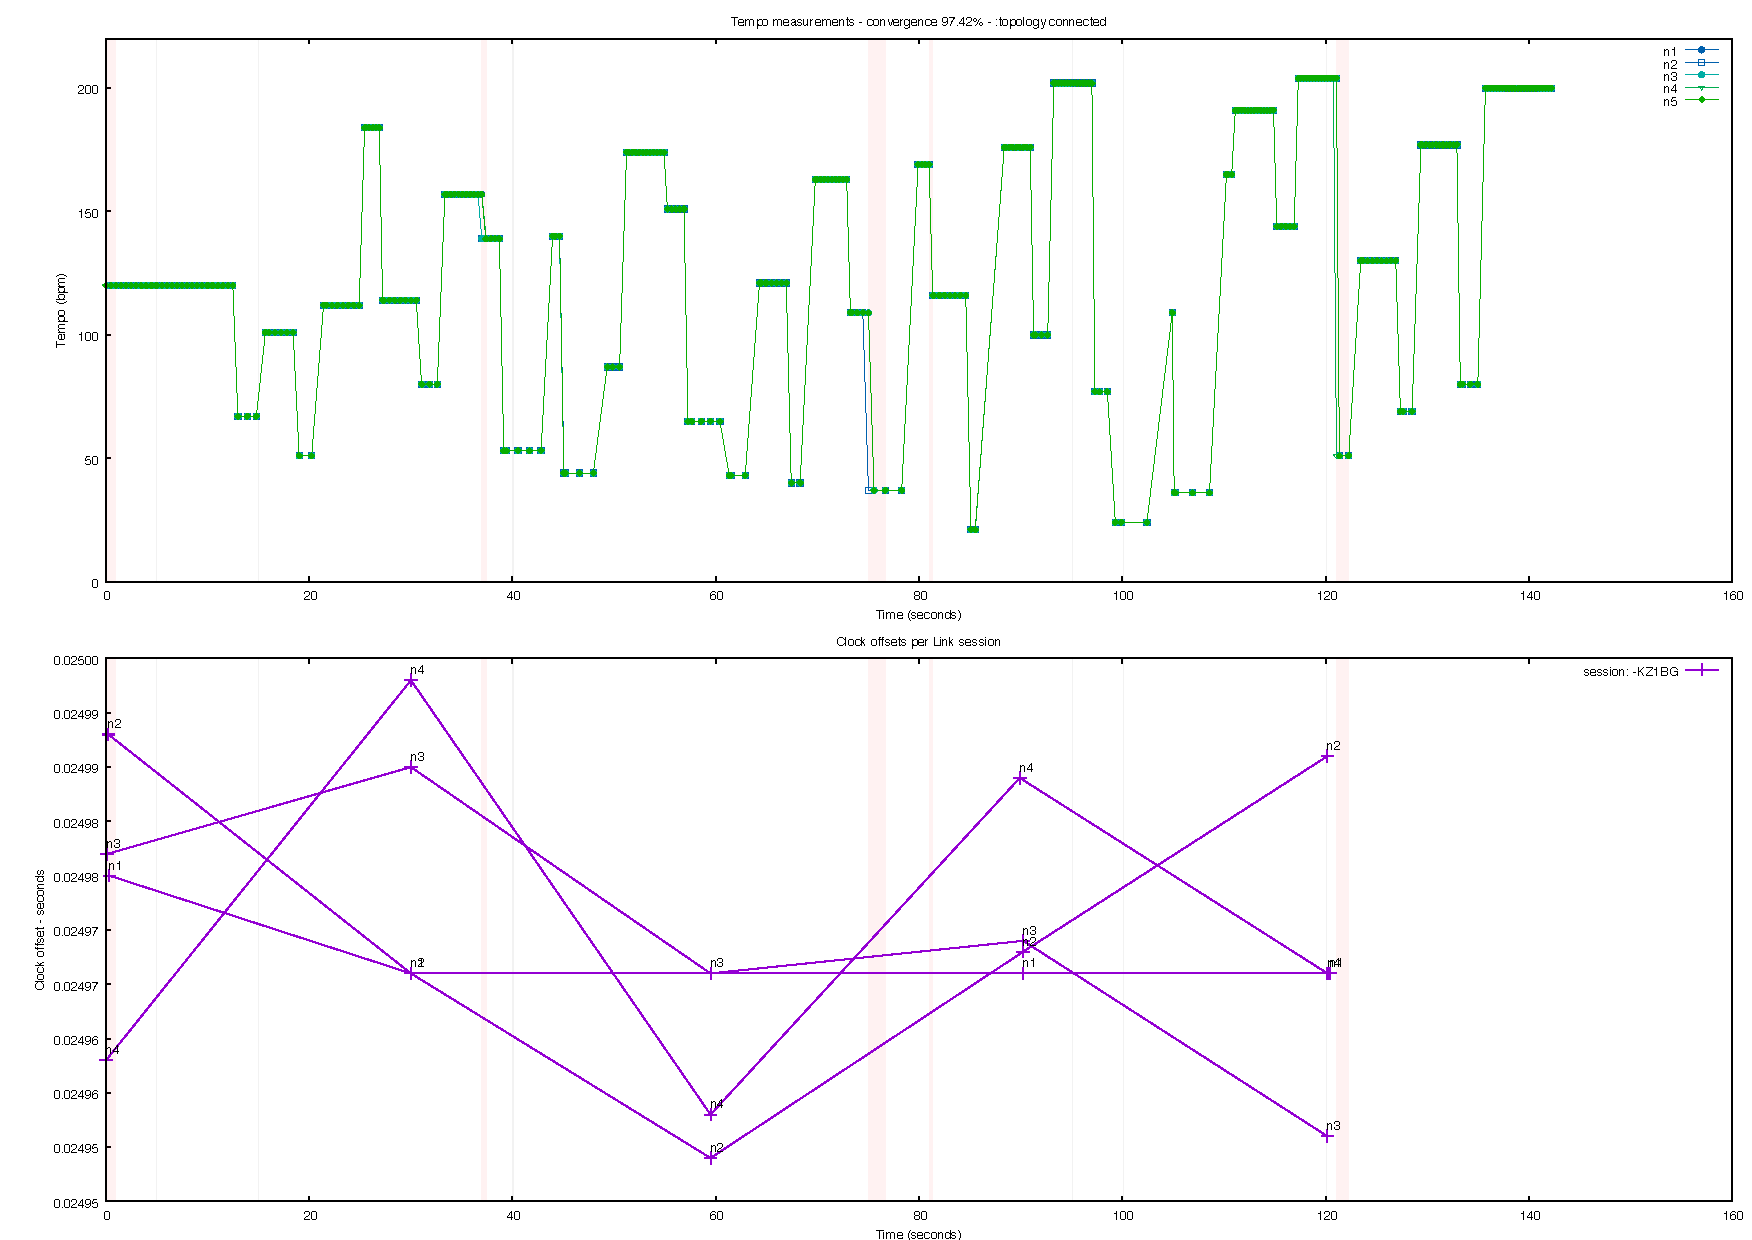
\includepdf[pages=-,angle=-90]{figures-for-publication/connected-no-delay/plot.pdf}
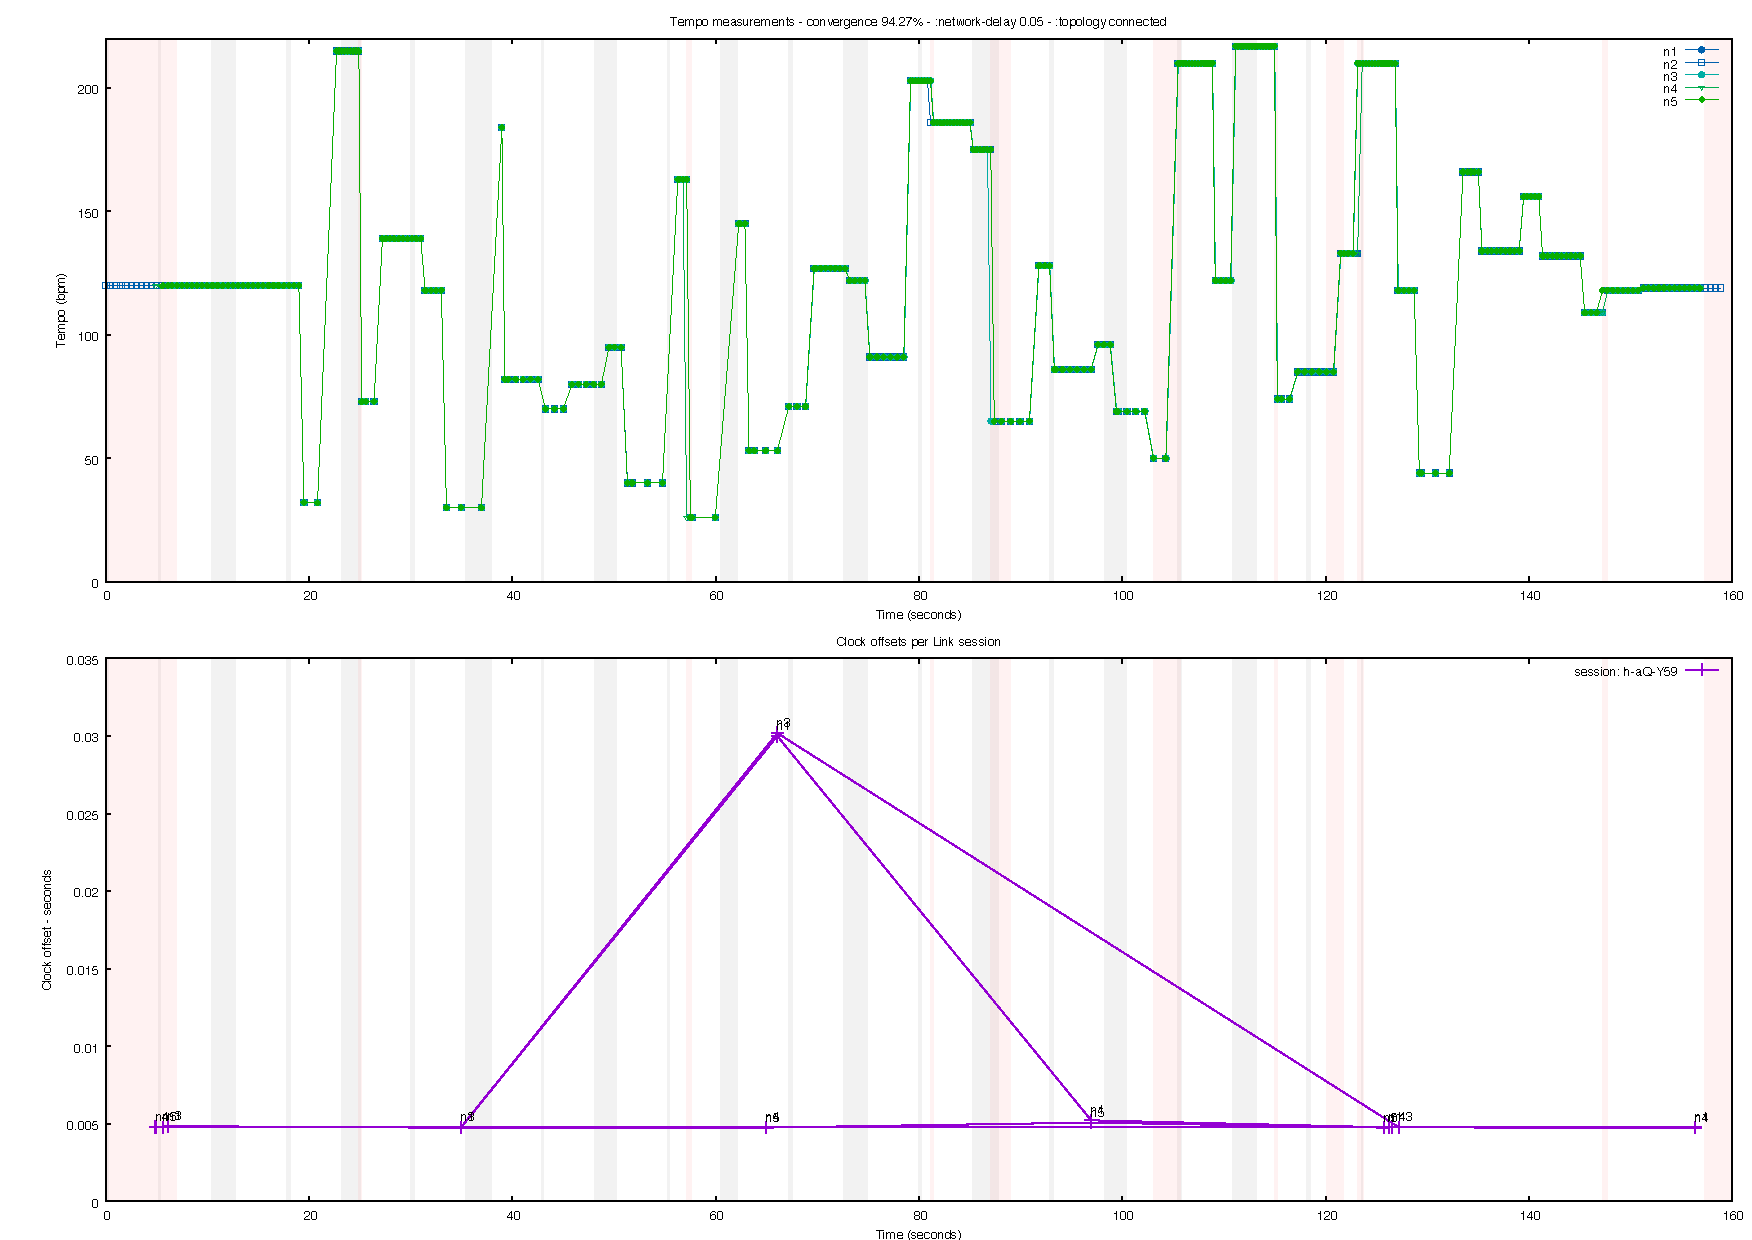
\includepdf[pages=-,angle=-90]{figures-for-publication/connected-50ms-delay/plot.pdf}
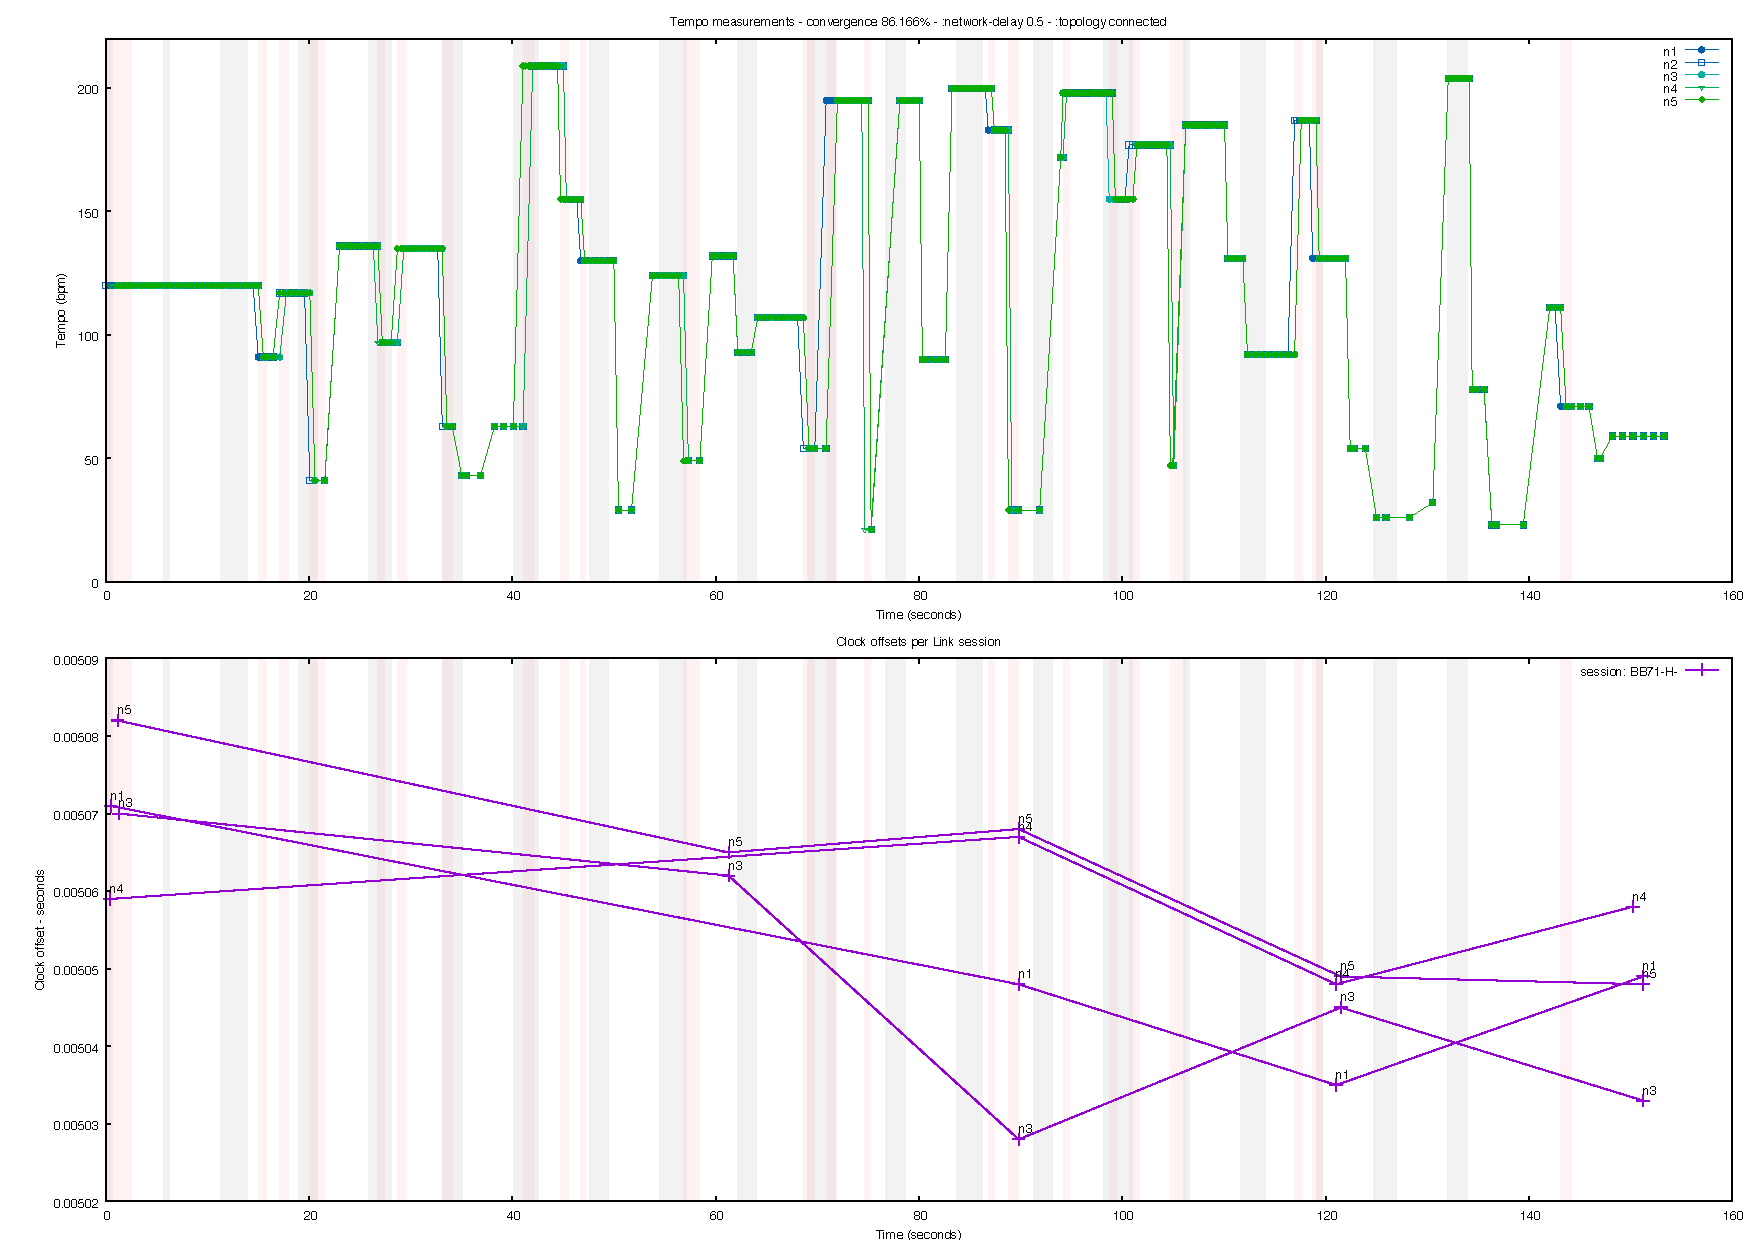
\includepdf[pages=-,angle=-90]{figures-for-publication/connected-500ms-delay/plot.pdf}
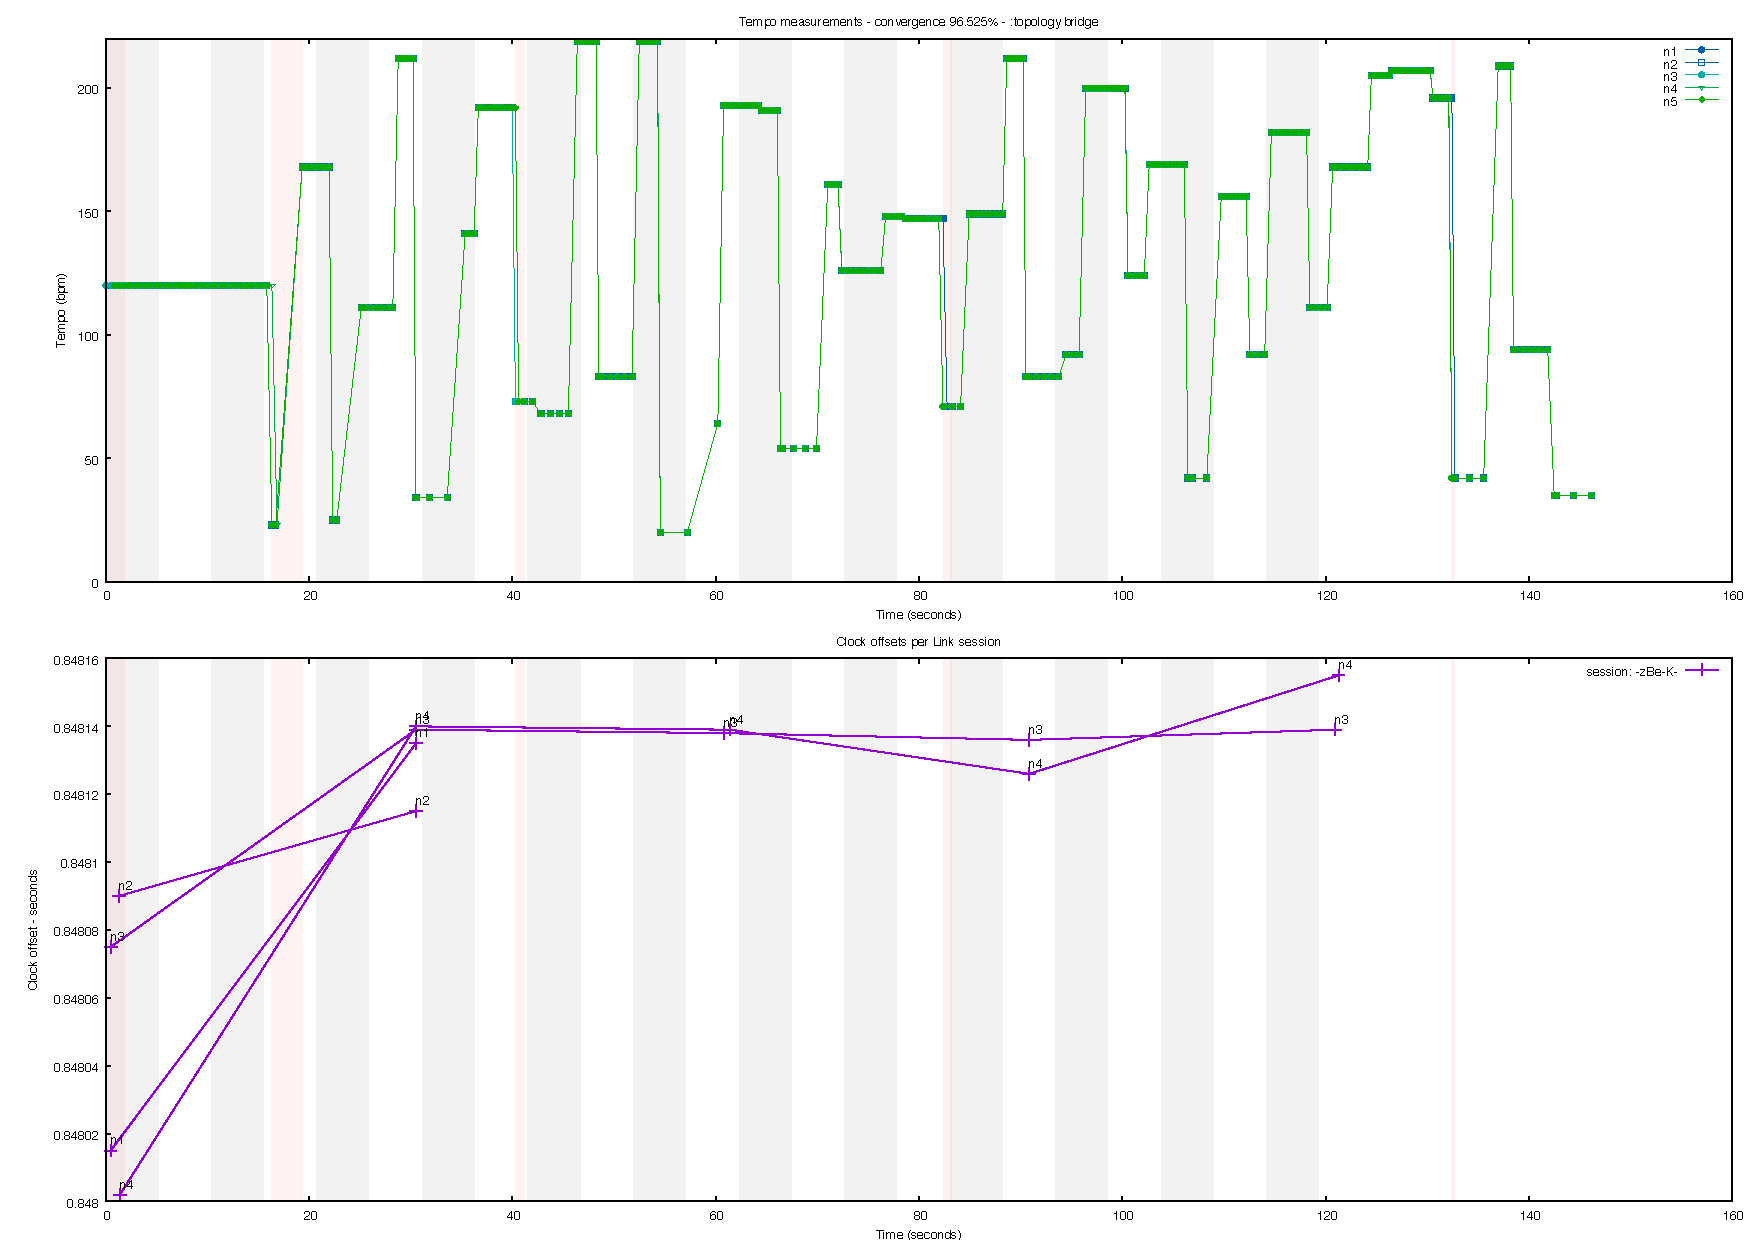
\includepdf[pages=-,angle=-90]{figures-for-publication/bridge-no-delay/plot.pdf}
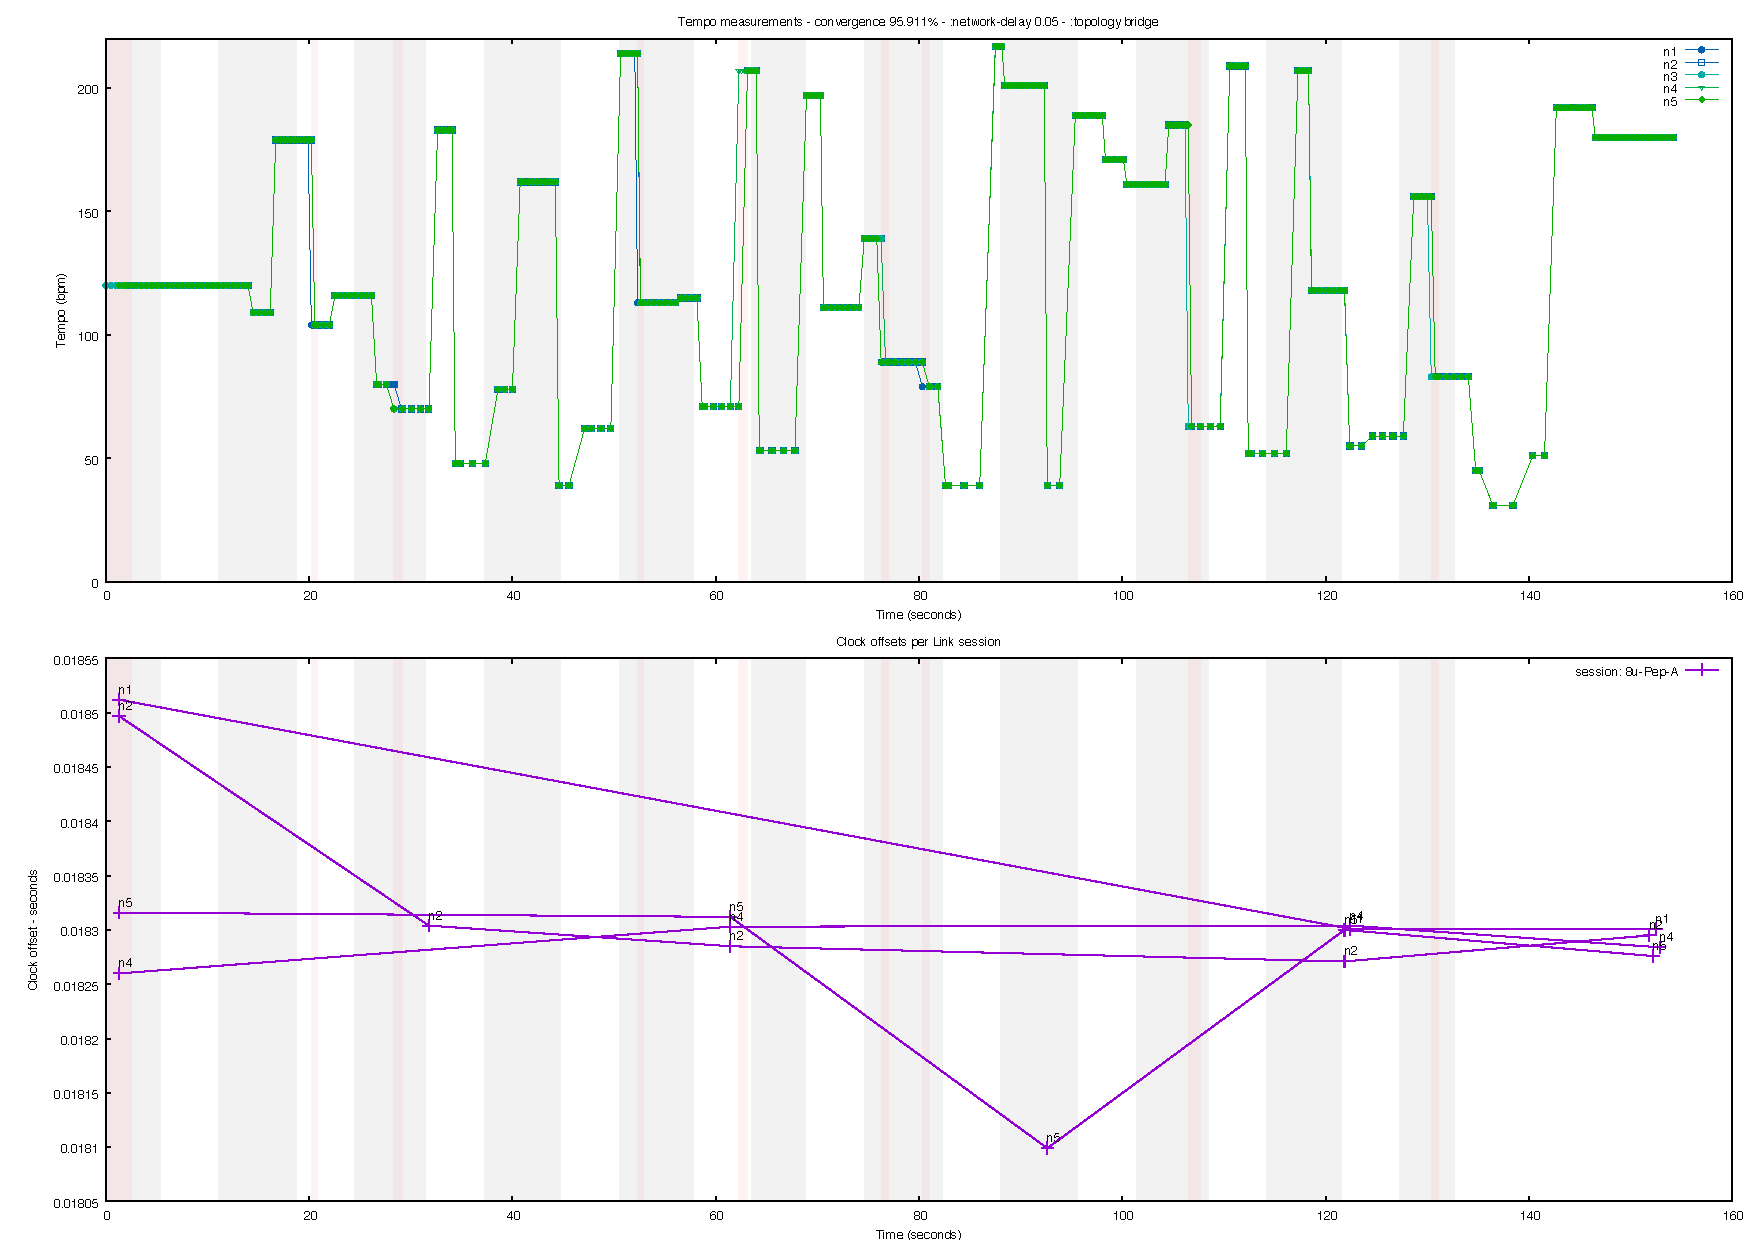
\includepdf[pages=-,angle=-90]{figures-for-publication/bridge-50ms-delay/plot.pdf}
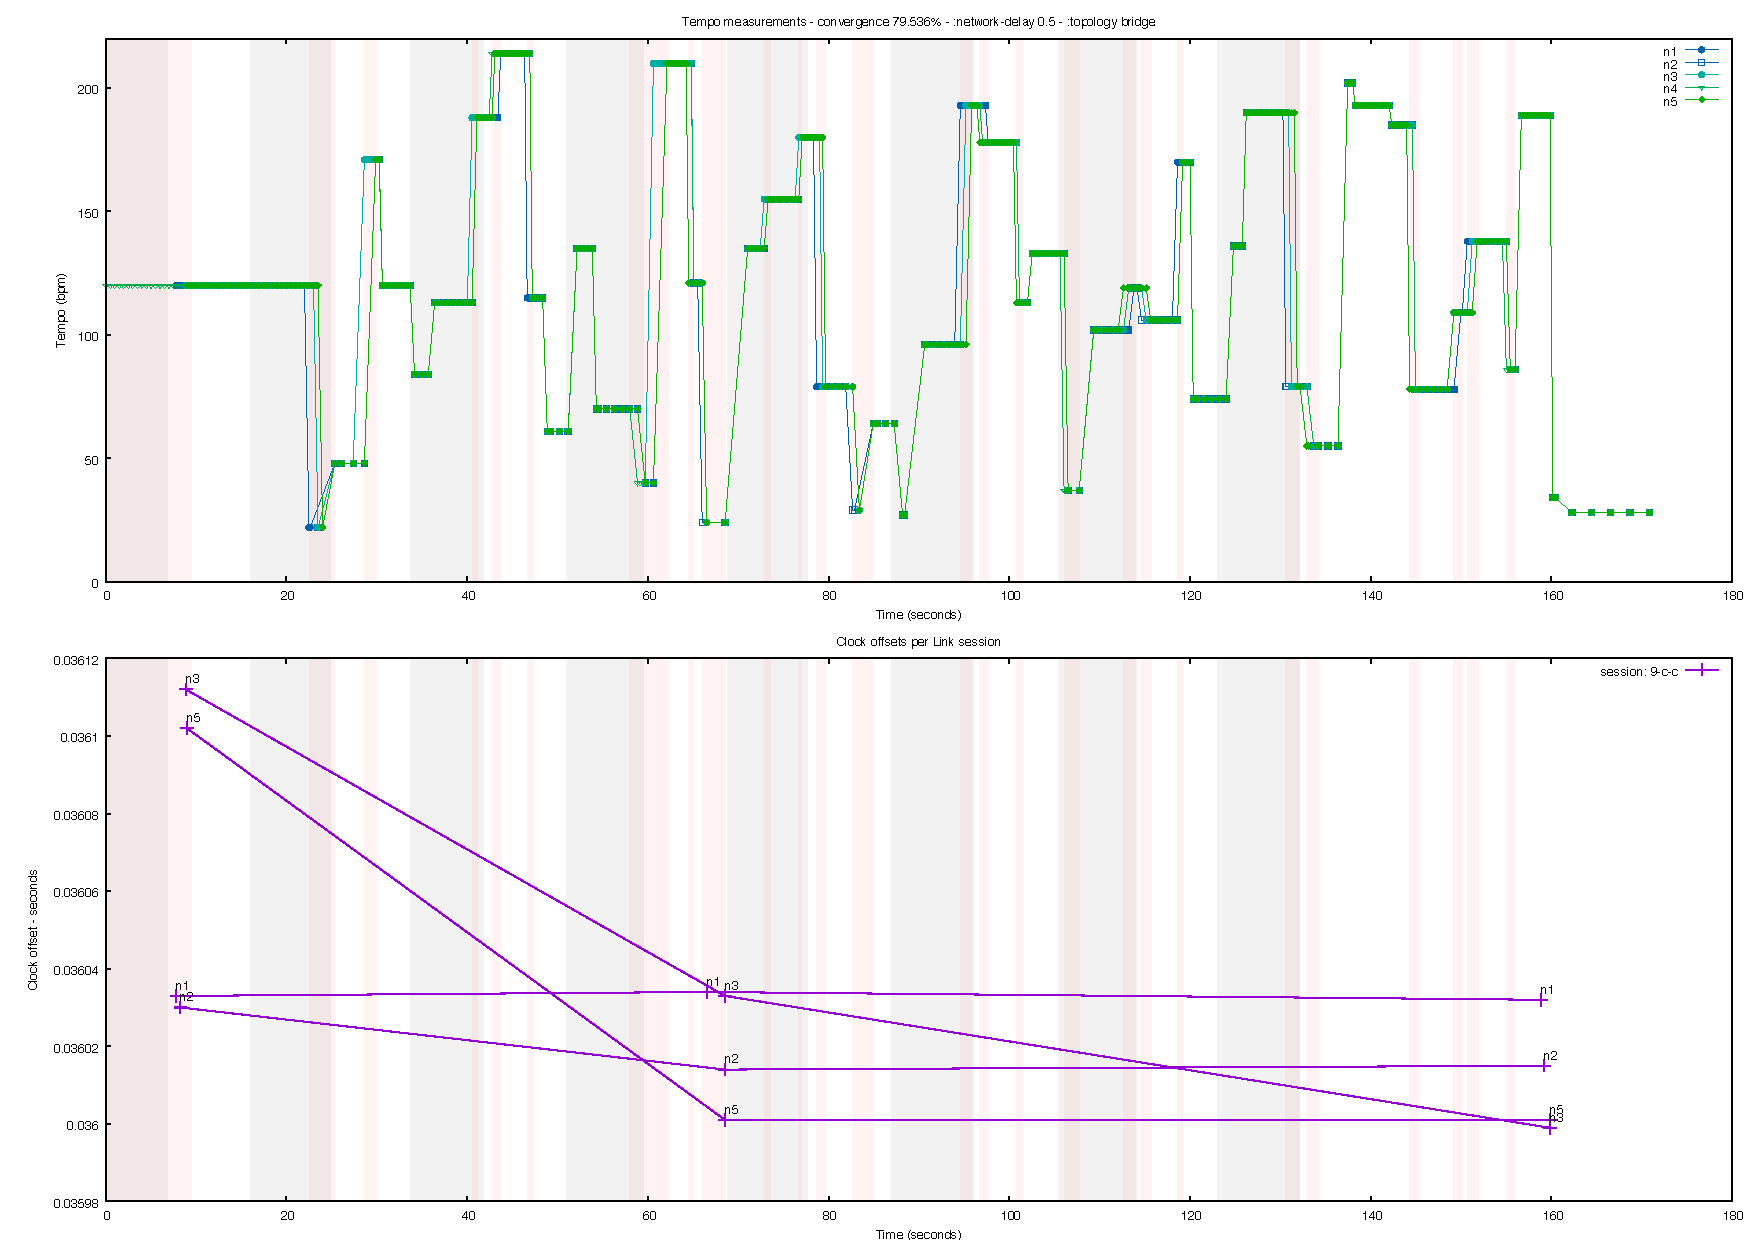
\includepdf[pages=-,angle=-90]{figures-for-publication/bridge-500ms-delay/plot.pdf}
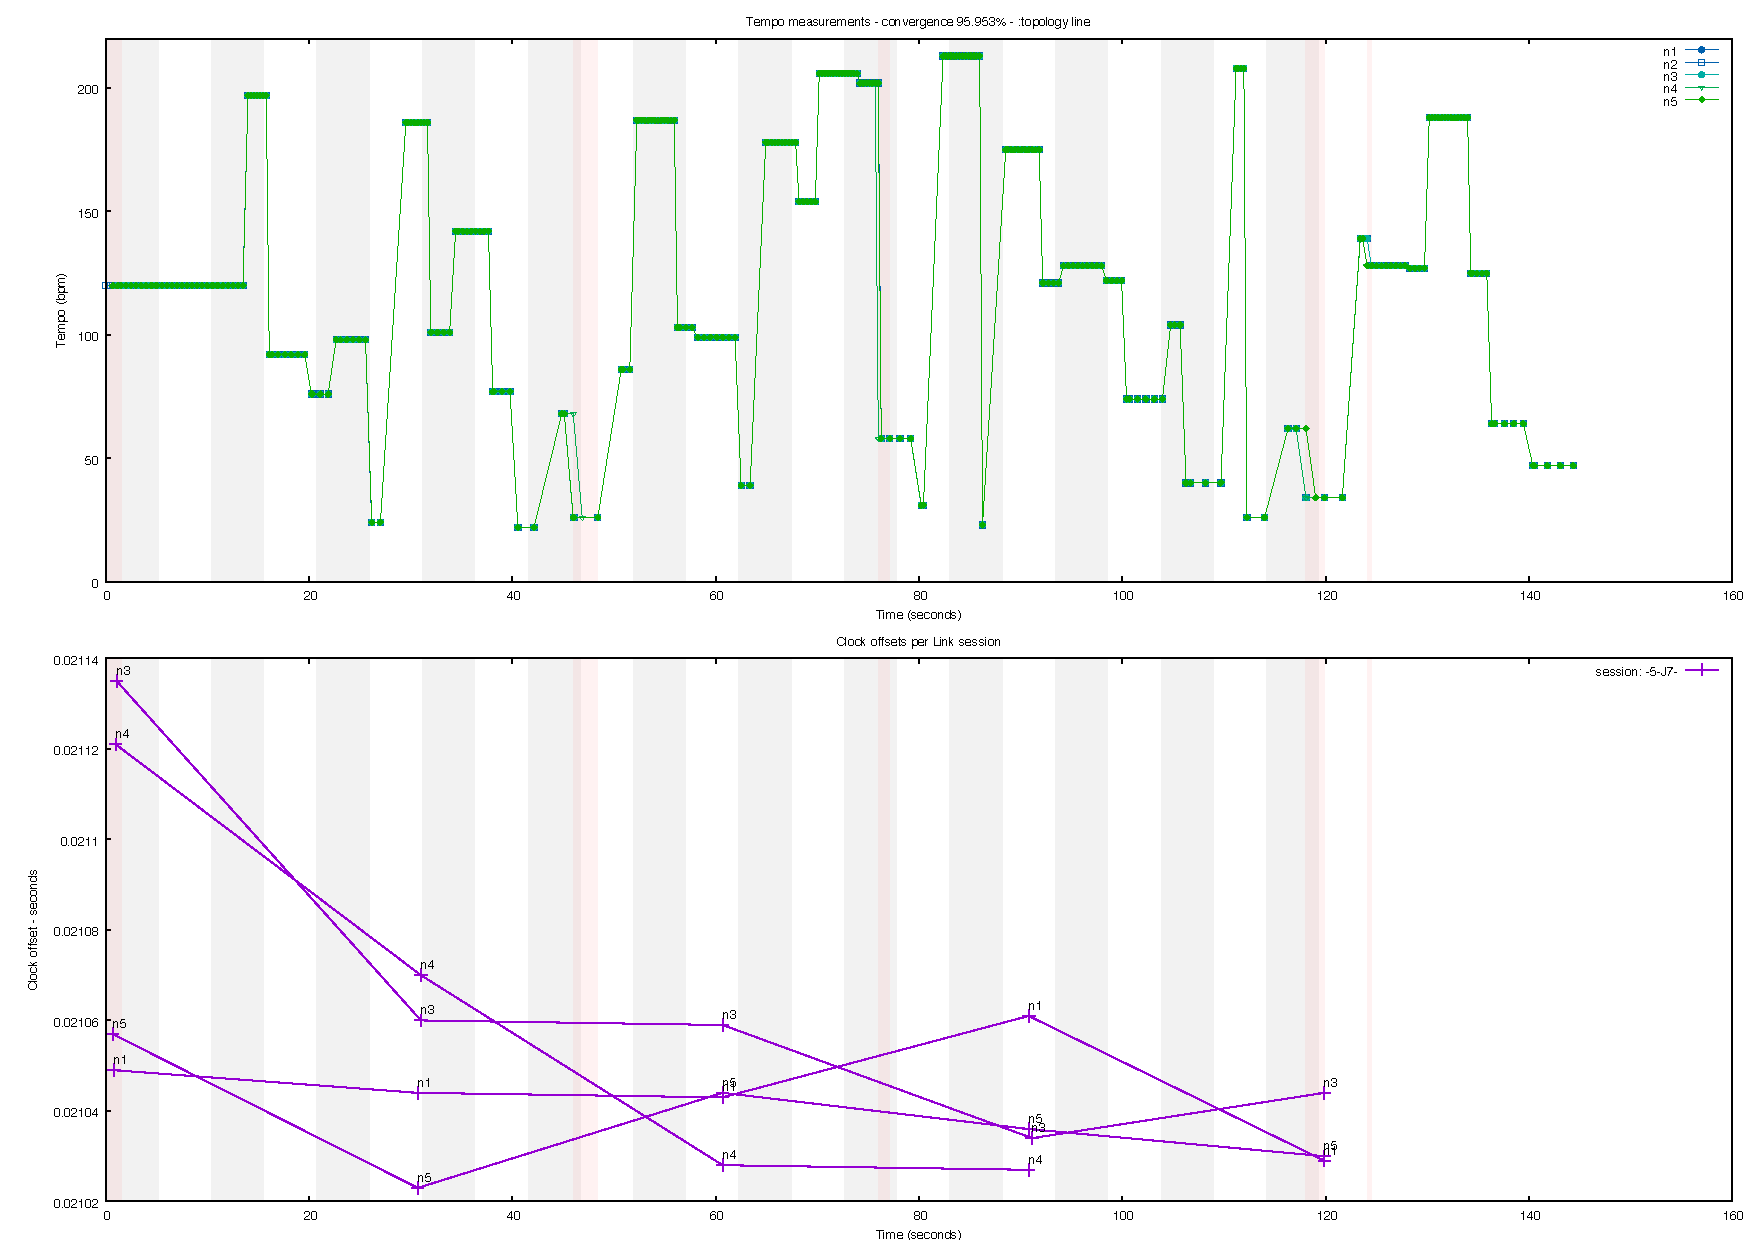
\includepdf[pages=-,angle=-90]{figures-for-publication/line-no-delay/plot.pdf}
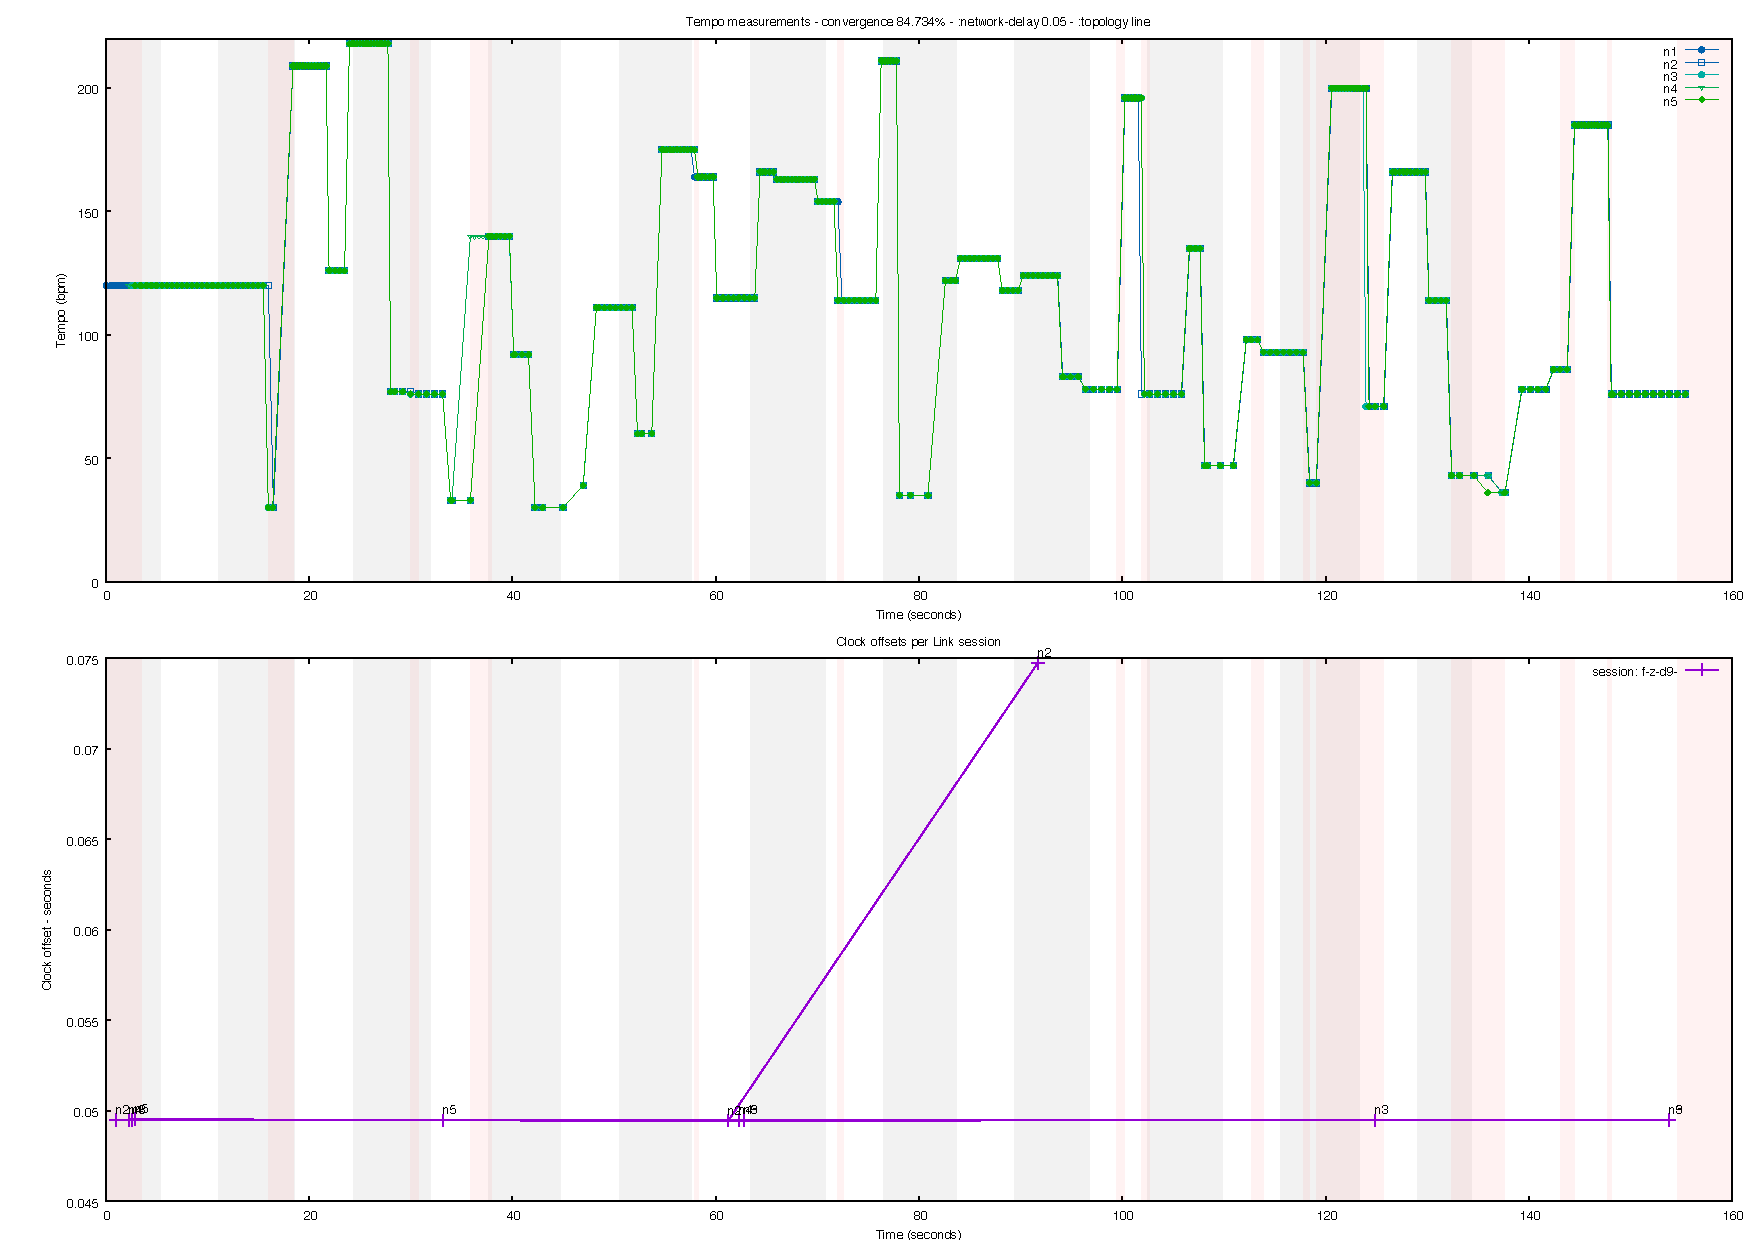
\includepdf[pages=-,angle=-90]{figures-for-publication/line-50ms-delay/plot.pdf}
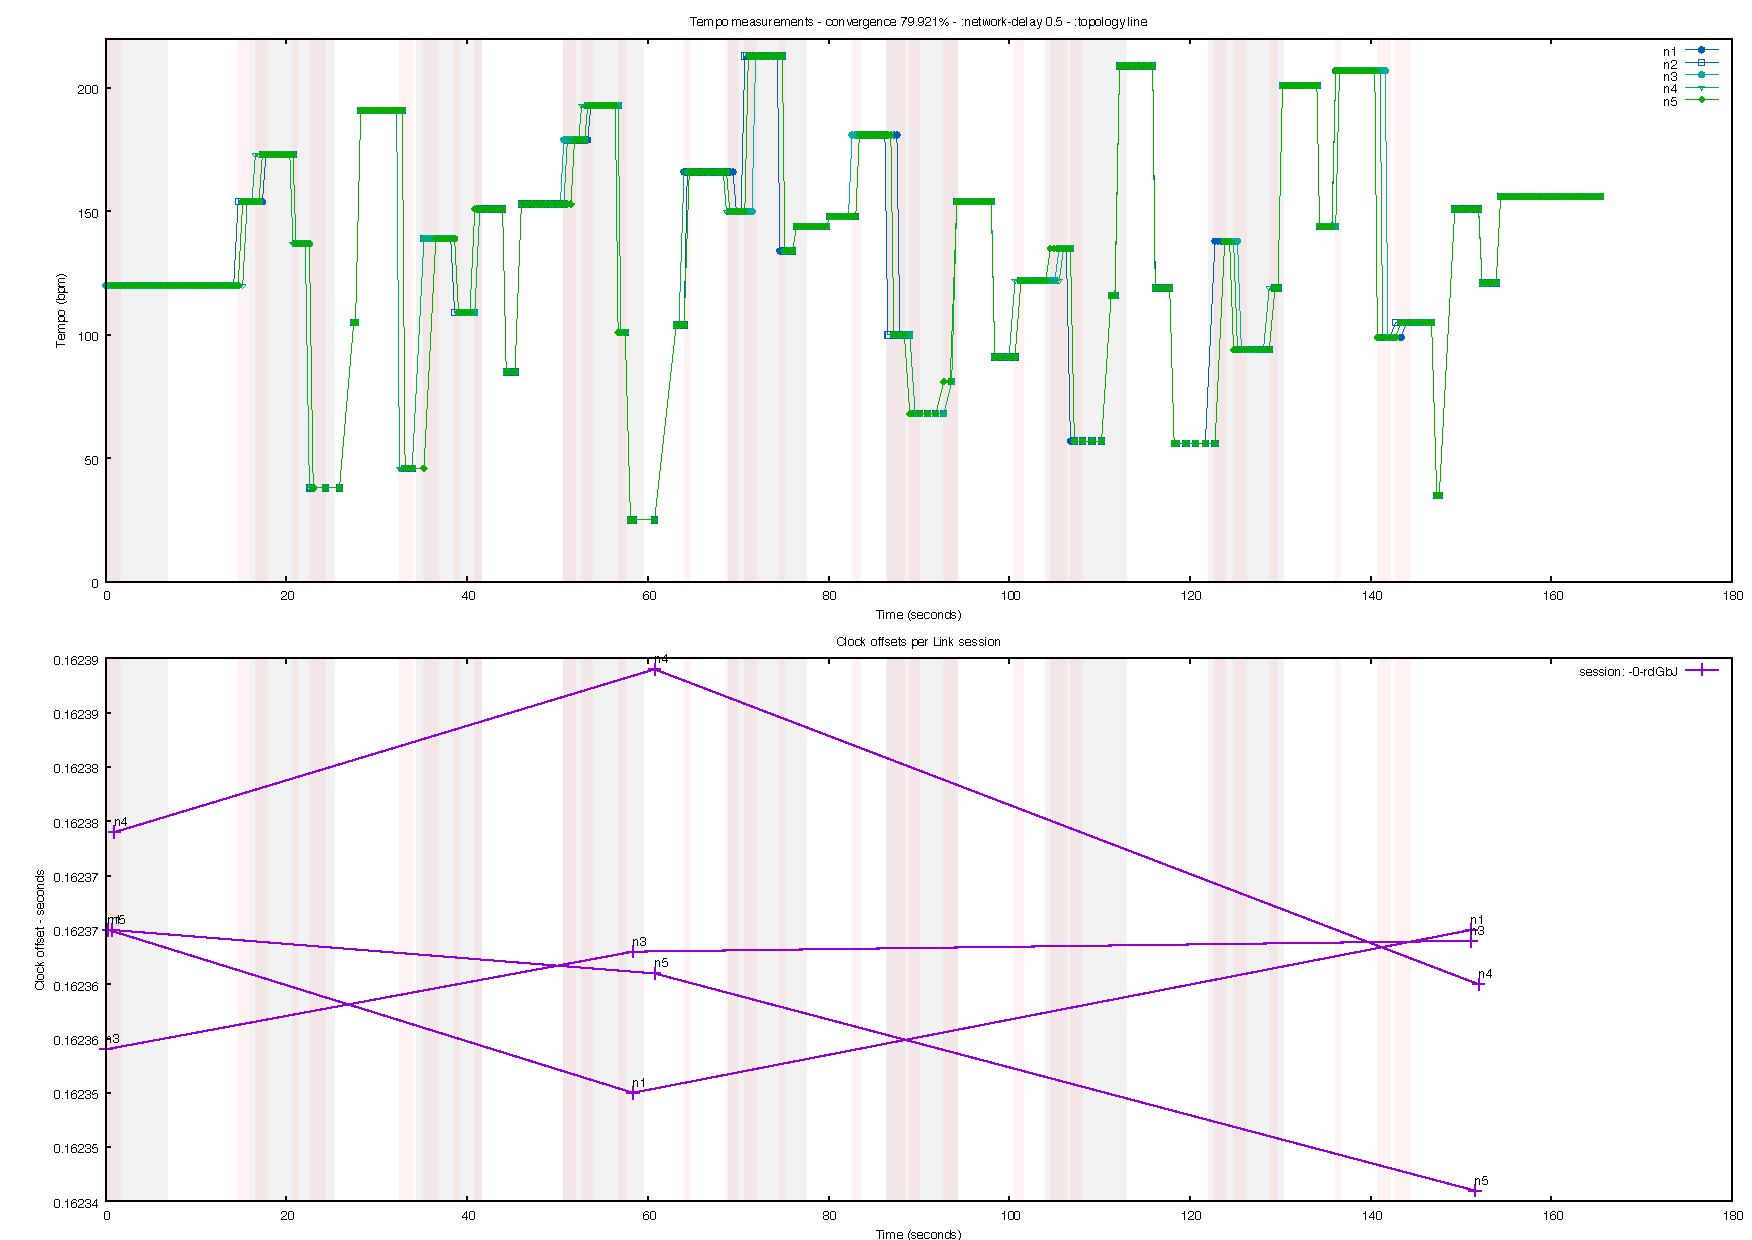
\includepdf[pages=-,angle=-90]{figures-for-publication/line-500ms-delay/plot.pdf}

\section{Analysis}

Resilient to different network conditions. Usually converges. Musical consistency has linear? falloff.

Talk about indeterminate divergence (missed statuses). Difficulty of measurements from a library with no configuration and little in the way of callbacks.

\subsection{Effects of delay distributions on clock synchronization}

Delay distributions and Kalman filtering - surprising results. Expected clock sync to track delays but apparently not.

Bandwidth measurements - difficult for partitions - maybe set partitions up first to see

\subsection{Identifying and triggering invalid states}

Ping/pong measurement has hardcoded cap of 50ms for RTT
Assuming RTT / 2 for latency calculation, this allows for max deviation of +/-25ms either side of leader
Anyway, the offset can vary by delta

Node A
send msgA tempo(120), t = 100
clock synchronization event - delta goes from 25ms to 0
send msgB tempo(140), t = 99.075
msgB is set locally (timestamp not checked for local updates)

Node B
recv msgA - newer than last tempo - set tempo = 120
recv msgB - reject (older when timestamps are compared)
broadcast state

Node A
recv state 120 with beat origin 100 - update? or not?

all neighbours behave the same, therefore 120 will be accepted and converged on however this seems sub-optimal.

If recv msgA is dropped/lost when received by Node C, then Node C will be tempo
= 140. If Node C retransmits with it's own beat origin (arbitrarily higher) then an inconsistent state is reached.


\section{Further work}

Generalize the work to other solutions.

Create CI testing for the Link library.

Suggest improvements to Link - Google nanosecond precision paper. Potential
uncertainty window around synchronization events. Configuration/visibility of
session information.

Integration into Sonic Pi. Windows compatibility.

\section{Conclusions}

\bibliographystyle{plain}
\bibliography{bibliography}

\appendix
\section{Self assessment}
\section{Running the tests}
\section{Configuring Jepsen to support other systems and tests}
\section{Code listings}
\section{Professional issues}
\section{Acknowledgements}

Open source code
Colleagues at Heroku
Salesforce for funding
Gregory and staff at RHUL
Em

\end{document}
